\documentclass{article}

\usepackage{graphicx}
\usepackage{amsmath}
\usepackage{fancyhdr}
\usepackage[sorting=none]{biblatex}
\usepackage[margin=1in]{geometry}
\usepackage[font={small,it}]{caption}
\usepackage{placeins}
\usepackage{xepersian}

%\DeclareMathOperator*{\btie}{\bowtie}
\addbibresource{bibliography.bib}
\settextfont[Scale=1.2]{B-NAZANIN.TTF}
\setlatintextfont[Scale=1]{Times New Roman}
\renewcommand{\baselinestretch}{1.5}
\pagestyle{fancy}
\fancyhf{}
\rhead{تکلیف اول آزمایشگاه سیستم عامل}
\lhead{\thepage}
\rfoot{علیرضا ابره فروش}
\lfoot{9816603}
\renewcommand{\headrulewidth}{1pt}
\renewcommand{\footrulewidth}{1pt}

\begin{document}
\begin{titlepage}
\begin{center}

\includegraphics[width=0.4\textwidth]{figures/IUT Logo.png}\\
        
\LARGE
\textbf{دانشگاه صنعتی اصفهان}\\
\textbf{دانشکده مهندسی برق و کامپیوتر}\\
        
\vfill
        
\huge
\textbf{عنوان: تکلیف چهارم درس ریزپردازنده}\\
        
\vfill
        
\LARGE
\textbf{نام و نام خانوادگی: علیرضا ابره فروش}\\
\textbf{شماره دانشجویی: 9816603}\\
\textbf{نیم\,سال تحصیلی: پاییز 1400}\\
\textbf{مدرّس: دکتر عارف کریمی افشار}\\
\end{center}
\end{titlepage}


%\tableofcontents
\newpage

\section{}
\subsection{}
\begin{figure}[ht]
    \centering
    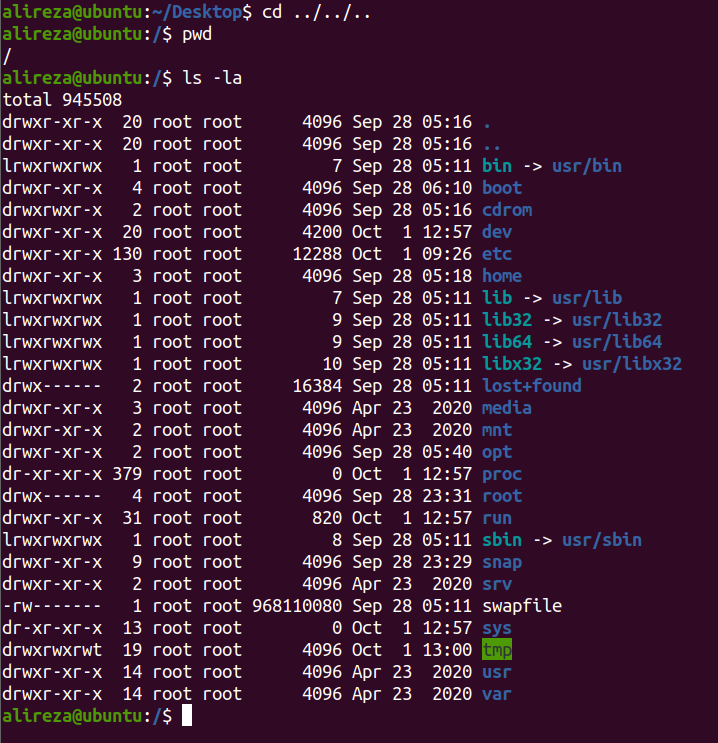
\includegraphics[width=0.95\textwidth]{figures/1.1.png}
    \caption
	{
دایرکتوری‌های
\lr{proc}
و
\lr{sys}
برای مالک اجازه
\lr{write}
ندارند.
	}
    \label{fig:fig1}
\end{figure}
\FloatBarrier

\subsection{}
\begin{figure}[ht]
    \centering
    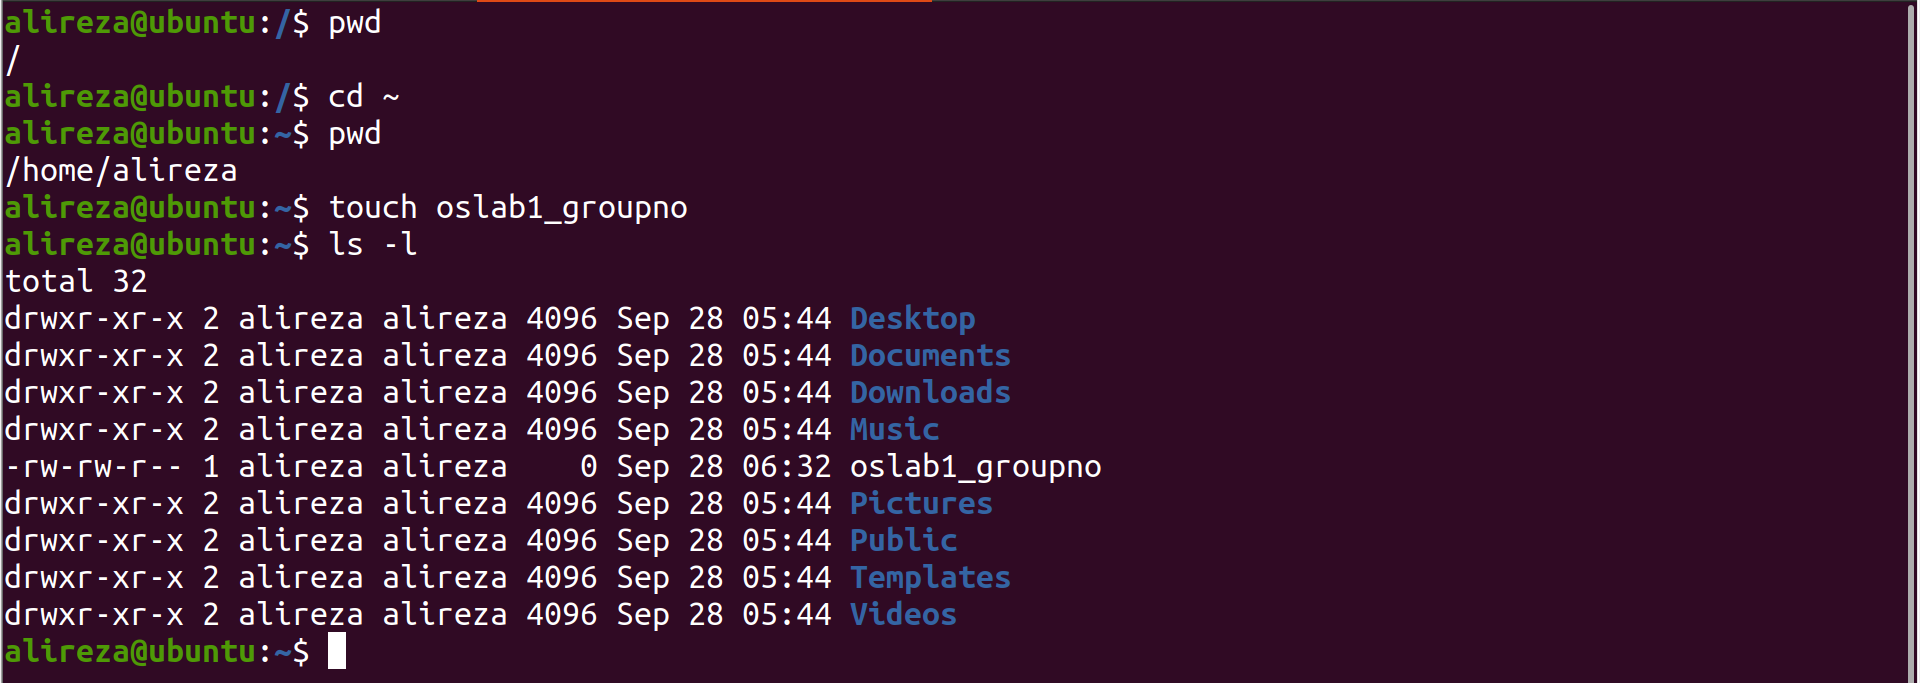
\includegraphics[width=1.0\textwidth]{figures/1.2.png}
    \caption
	{
زمان آخرین دسترسی به فایل 06:32 می‌باشد.
	}
    \label{fig:fig1}
\end{figure}
\FloatBarrier

\subsection{}
\begin{figure}[ht]
    \centering
    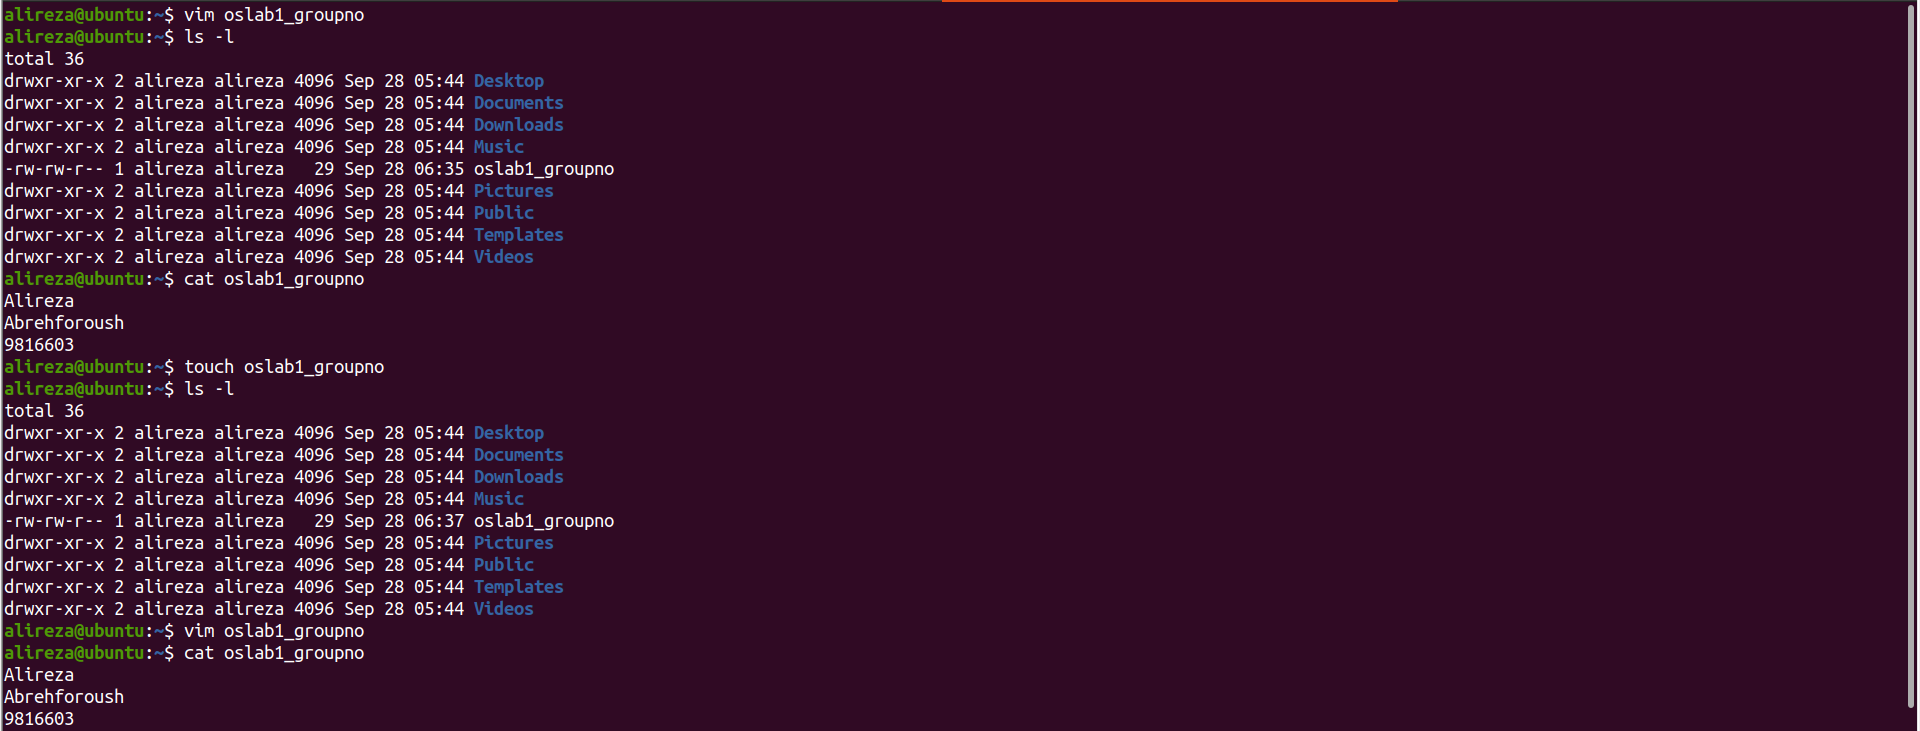
\includegraphics[width=1.0\textwidth]{figures/1.3.png}
    \caption
	{
زمان آخرین دسترسی به فایل 06:35 می‌باشد.
	}
    \label{fig:fig1}
\end{figure}
\FloatBarrier

\subsection{}
\begin{figure}[ht]
    \centering
    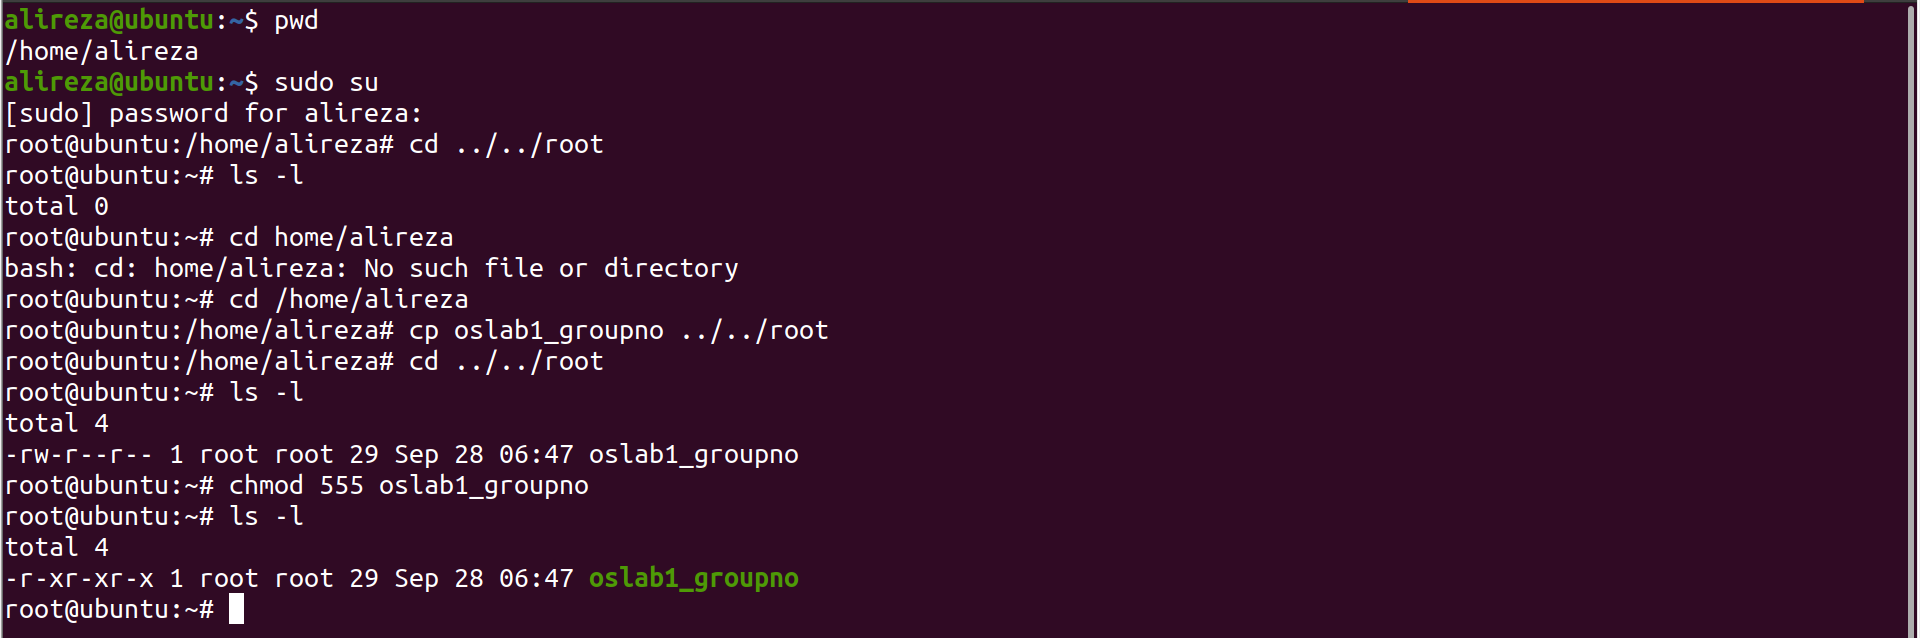
\includegraphics[width=1.0\textwidth]{figures/1.4.png}
    \caption{}
    \label{fig:fig1}
\end{figure}
\FloatBarrier

\section{}
\begin{figure}[ht]
    \centering
    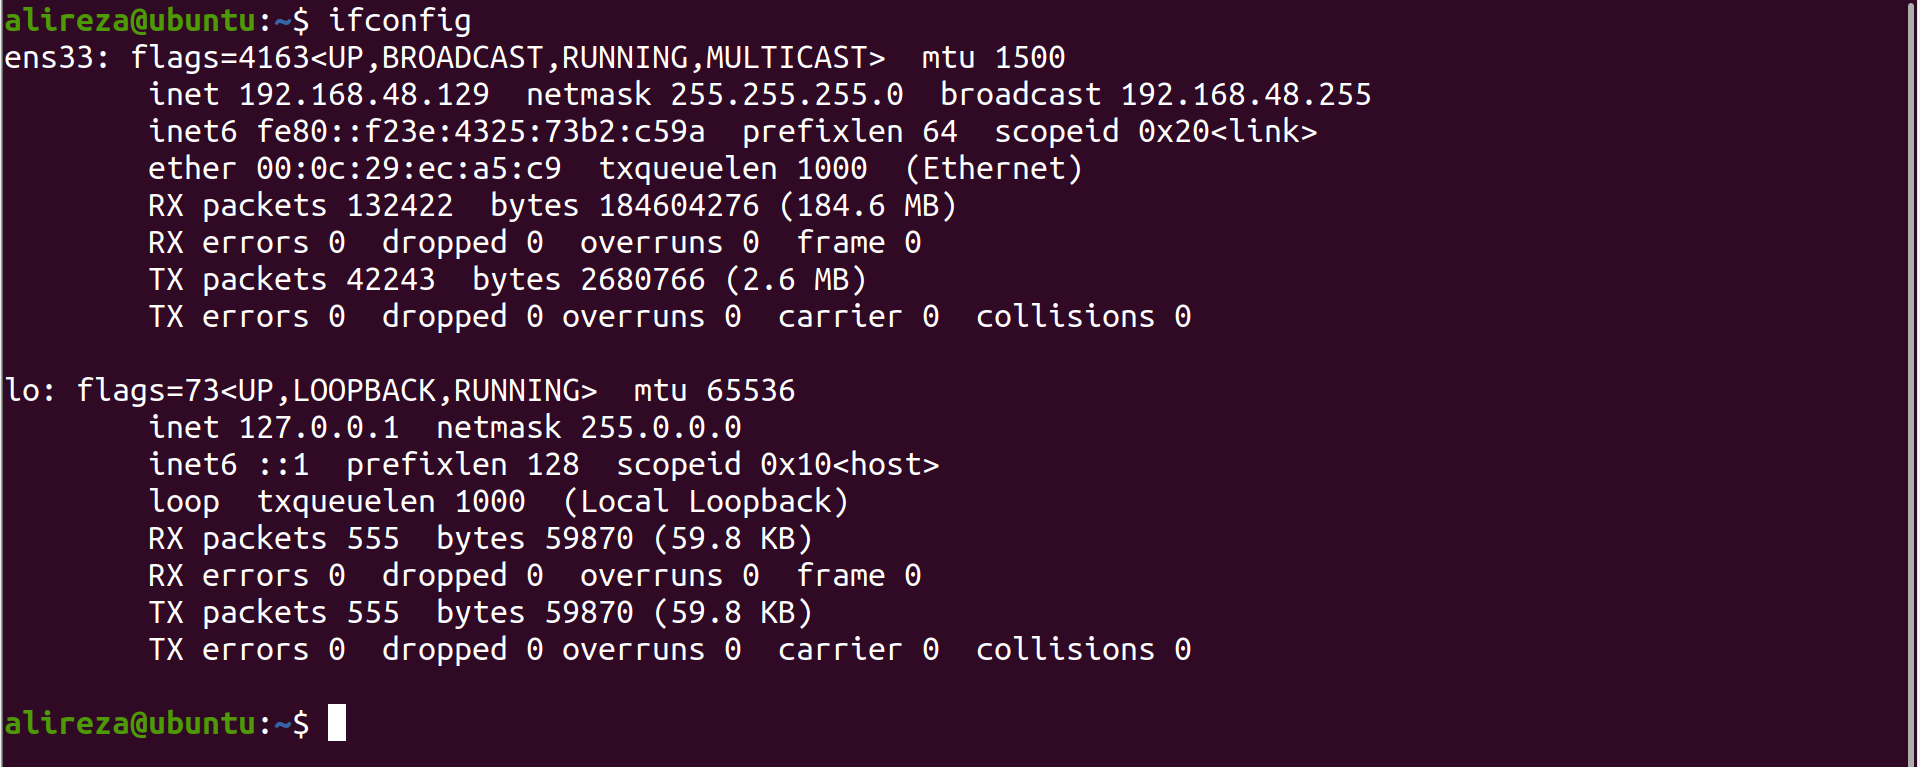
\includegraphics[width=1.0\textwidth]{figures/2.png}
    \caption{}
    \label{fig:fig1}
\end{figure}
\FloatBarrier


\section{}
\begin{figure}[ht]
    \centering
    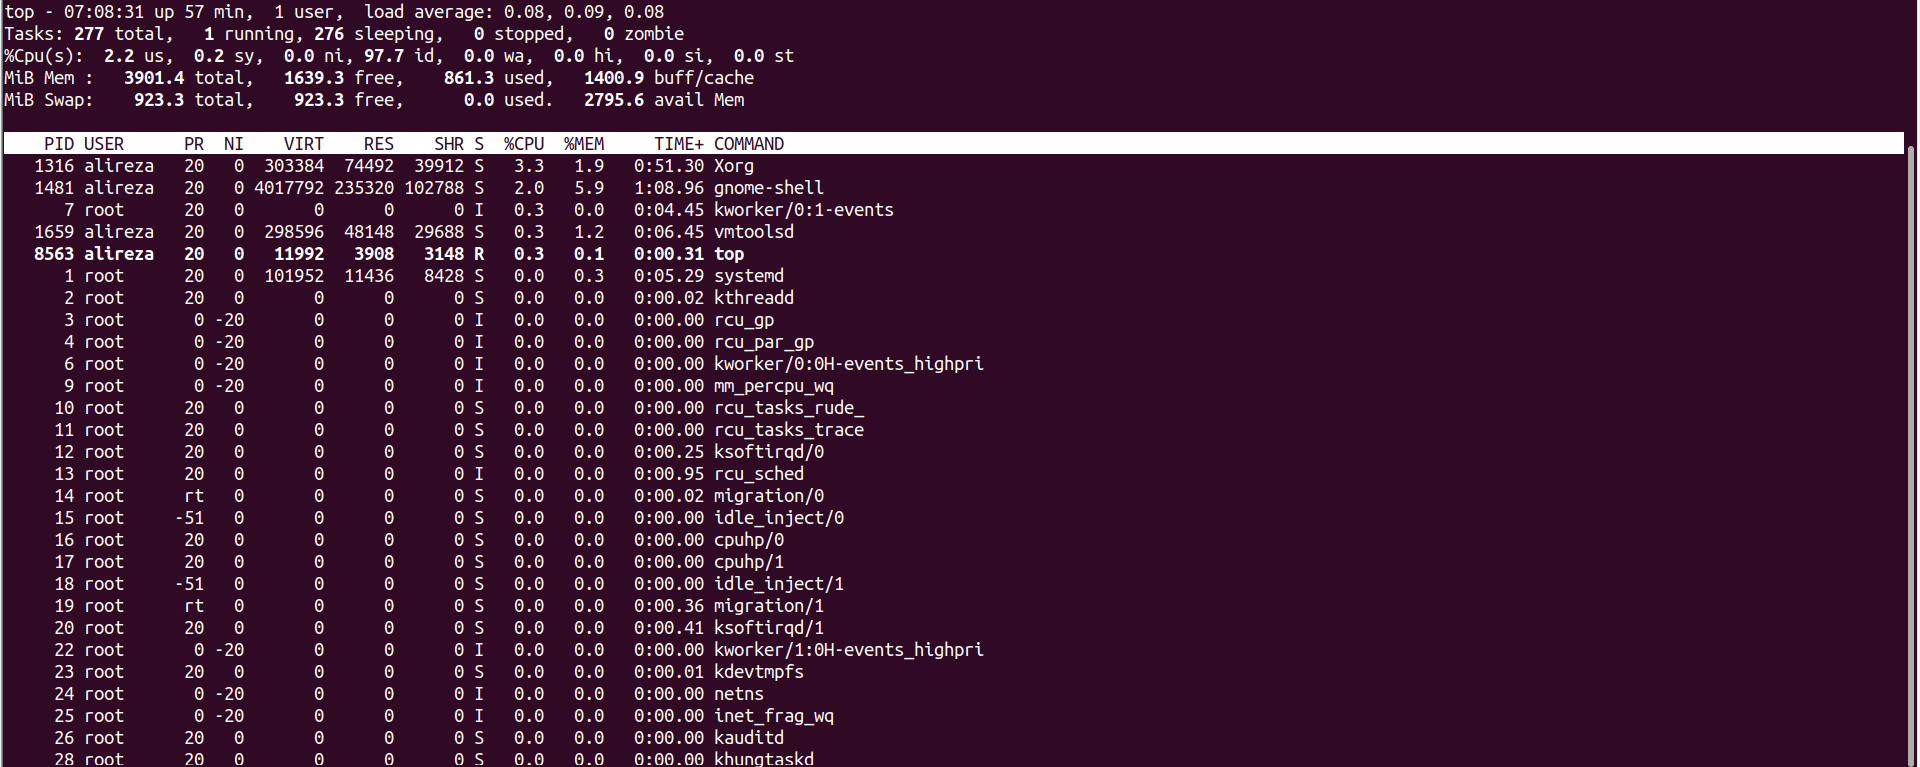
\includegraphics[width=1.0\textwidth]{figures/3.png}
    \caption
	{
\lr{Xorg}
و
\lr{gnome-shell}
و
\lr{vmtoolsd}
سه برنامه درحال اجرا هستند که بیشترین مقدار حافظه اصلی را استفاده می‌کنند.
	}
    \label{fig:fig1}
\end{figure}
\FloatBarrier

\section{}
\subsection{}
\begin{figure}[ht]
    \centering
    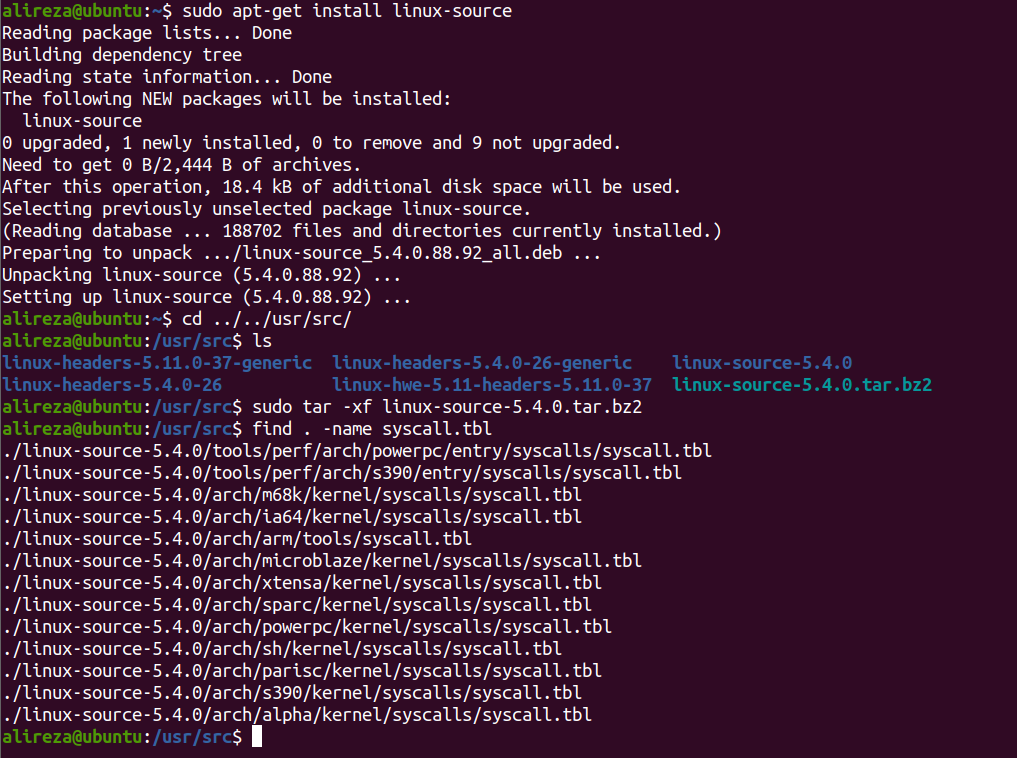
\includegraphics[width=1.0\textwidth]{figures/a.png}
    \caption{}
    \label{fig:fig1}
\end{figure}
\FloatBarrier

\subsection{}
7 تا مربوط به
\lr{write}
است.
\begin{figure}[ht]
    \centering
    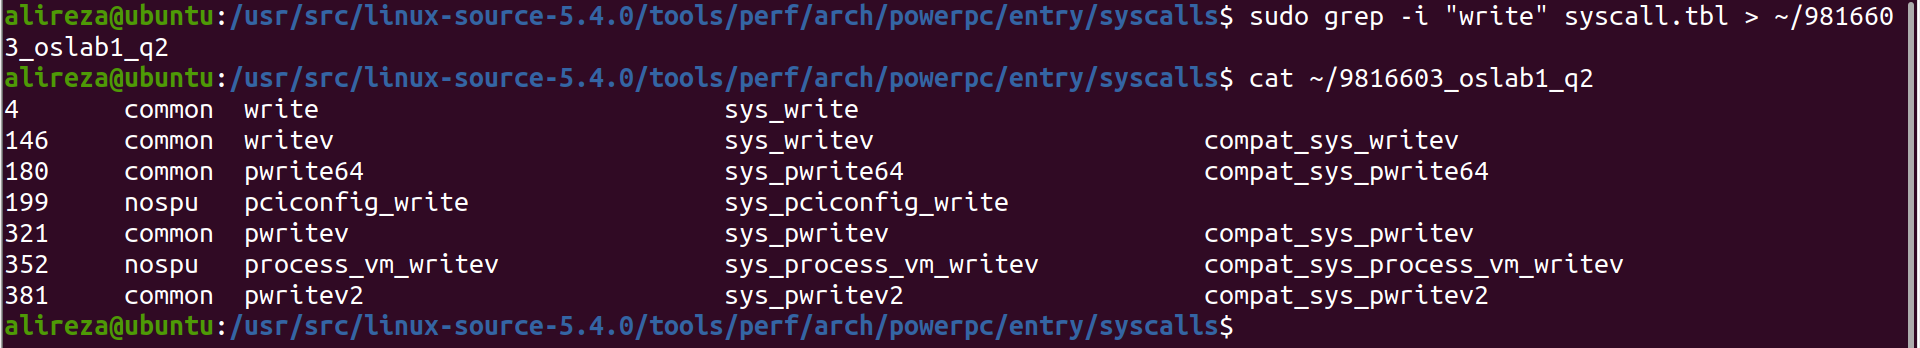
\includegraphics[width=1.0\textwidth]{figures/b.png}
    \caption{}
    \label{fig:fig1}
\end{figure}
\FloatBarrier

\section{}
\begin{figure}[ht]
    \centering
    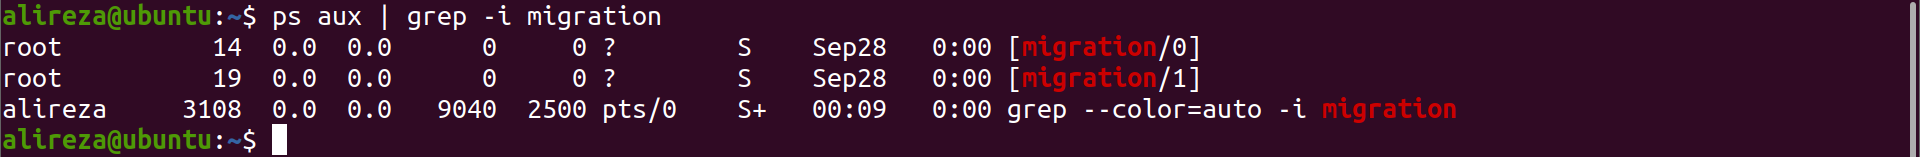
\includegraphics[width=1.0\textwidth]{figures/5.png}
    \caption{}
    \label{fig:fig1}
\end{figure}
\FloatBarrier

\section{}
\begin{figure}[ht]
    \centering
    
\includegraphics[width=1.0\textwidth]{figures/6.png}
    \caption{}
    \label{fig:fig1}
\end{figure}
\FloatBarrier

\section{}
\begin{figure}[ht]
    \centering
    
\includegraphics[width=1.0\textwidth]{figures/7.png}
    \caption{}
    \label{fig:fig1}
\end{figure}
\FloatBarrier

\section{}
\begin{figure}[ht]
    \centering
    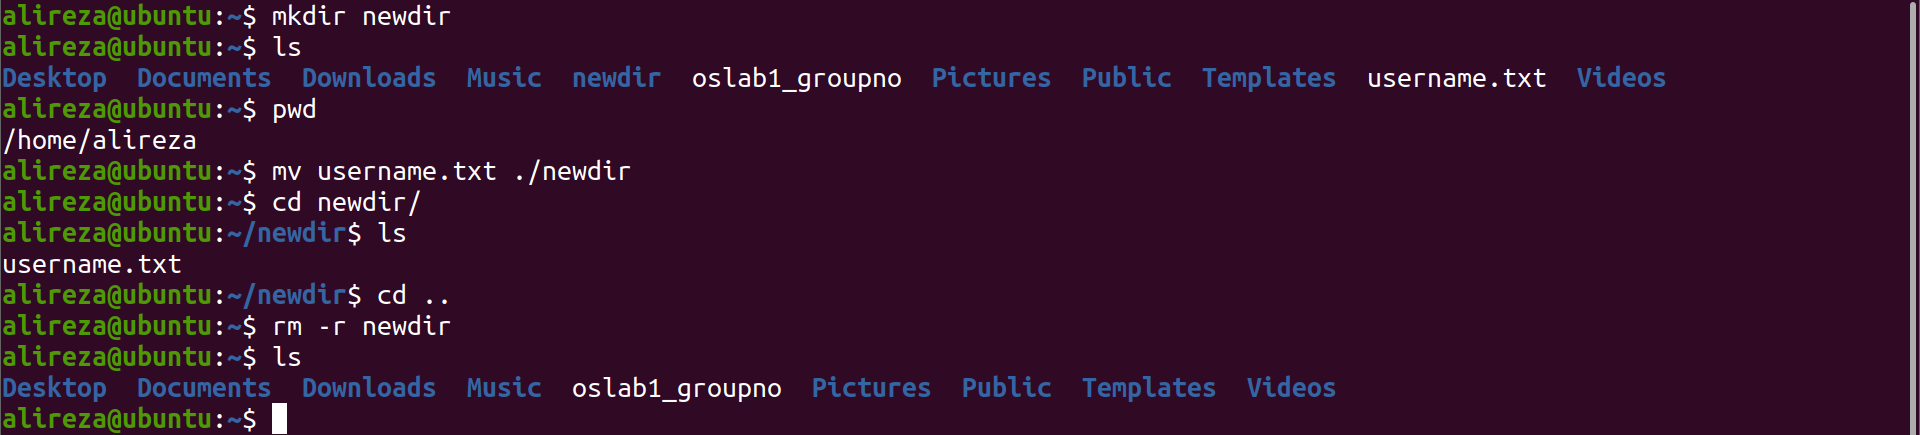
\includegraphics[width=1.0\textwidth]{figures/8.png}
    \caption{}
    \label{fig:fig1}
\end{figure}
\FloatBarrier

\section*{منابع}
\renewcommand{\section}[2]{}%
\begin{thebibliography}{99} % assumes less than 100 references
%چنانچه مرجع فارسی نیز داشته باشید باید دستور فوق را فعال کنید و مراجع فارسی خود را بعد از این دستور وارد کنید


\begin{LTRitems}

\resetlatinfont

\bibitem{b1} https://www.geeksforgeeks.org
\end{LTRitems}

\end{thebibliography}


\end{document}
